\label{user-registration}
\subsubsection{Purpose}
Any user can subscribe through the web application or the mobile app.

In both cases the user has to fill a registration form and must agree to the personal data policy according to his/her country privacy laws, otherwise the registration request shall be aborted.

As soon as the user has submitted all the data, the system verifies the consistency of the information and a confirmation mail is sent to check the availability of the email-address.  After this last check the registration ends successfully.

The system has two kind of registration forms (for the two kinds of registered users): one for passengers and one for taxi drivers.

The taxi driver registration is more restrictive and requires more user information.
The system registers a user that claims to be a taxi driver only if he/she is able to prove it with a currently valid taxi license.


\subsubsection{Scenario 1}
Alice, a normal citizen without a car, has just discovered the existence of myTaxiService web application and she wants to use it.
She opens the homepage of myTaxiService on the website and clicks on ``passenger registration''.

She gives all the information required and authorises the personal data treatment.

The system verifies the submitted information and sends a confirmation mail.
Alice checks the mailbox, opens the mail and clicks on the ``confirm e-mail'' link.

The system informs Alice that the registration succeeded.

\subsubsection{Scenario 2}
Bob is a taxi driver that wants to subscribe to myTaxiService application.
He downloads the mobile application from his phone app-store and once he opens it, he selects ``taxi driver registration''.
He fills the form, enters his license ID and authorises the personal data treatment.

However he forgets to write his phone number on the form so the system warns him about the forgetfulness.
Only after the complete and correct filling of the form, and the personal data treatment authorisation, the registration is one step near the successfully end.

The system verifies the information submitted and sends a confirmation mail.
Bob checks the mailbox, opens the mail and clicks on ``confirm e-mail''.

The system informs Bob that the registration has ended successfully.

\begin{figure}
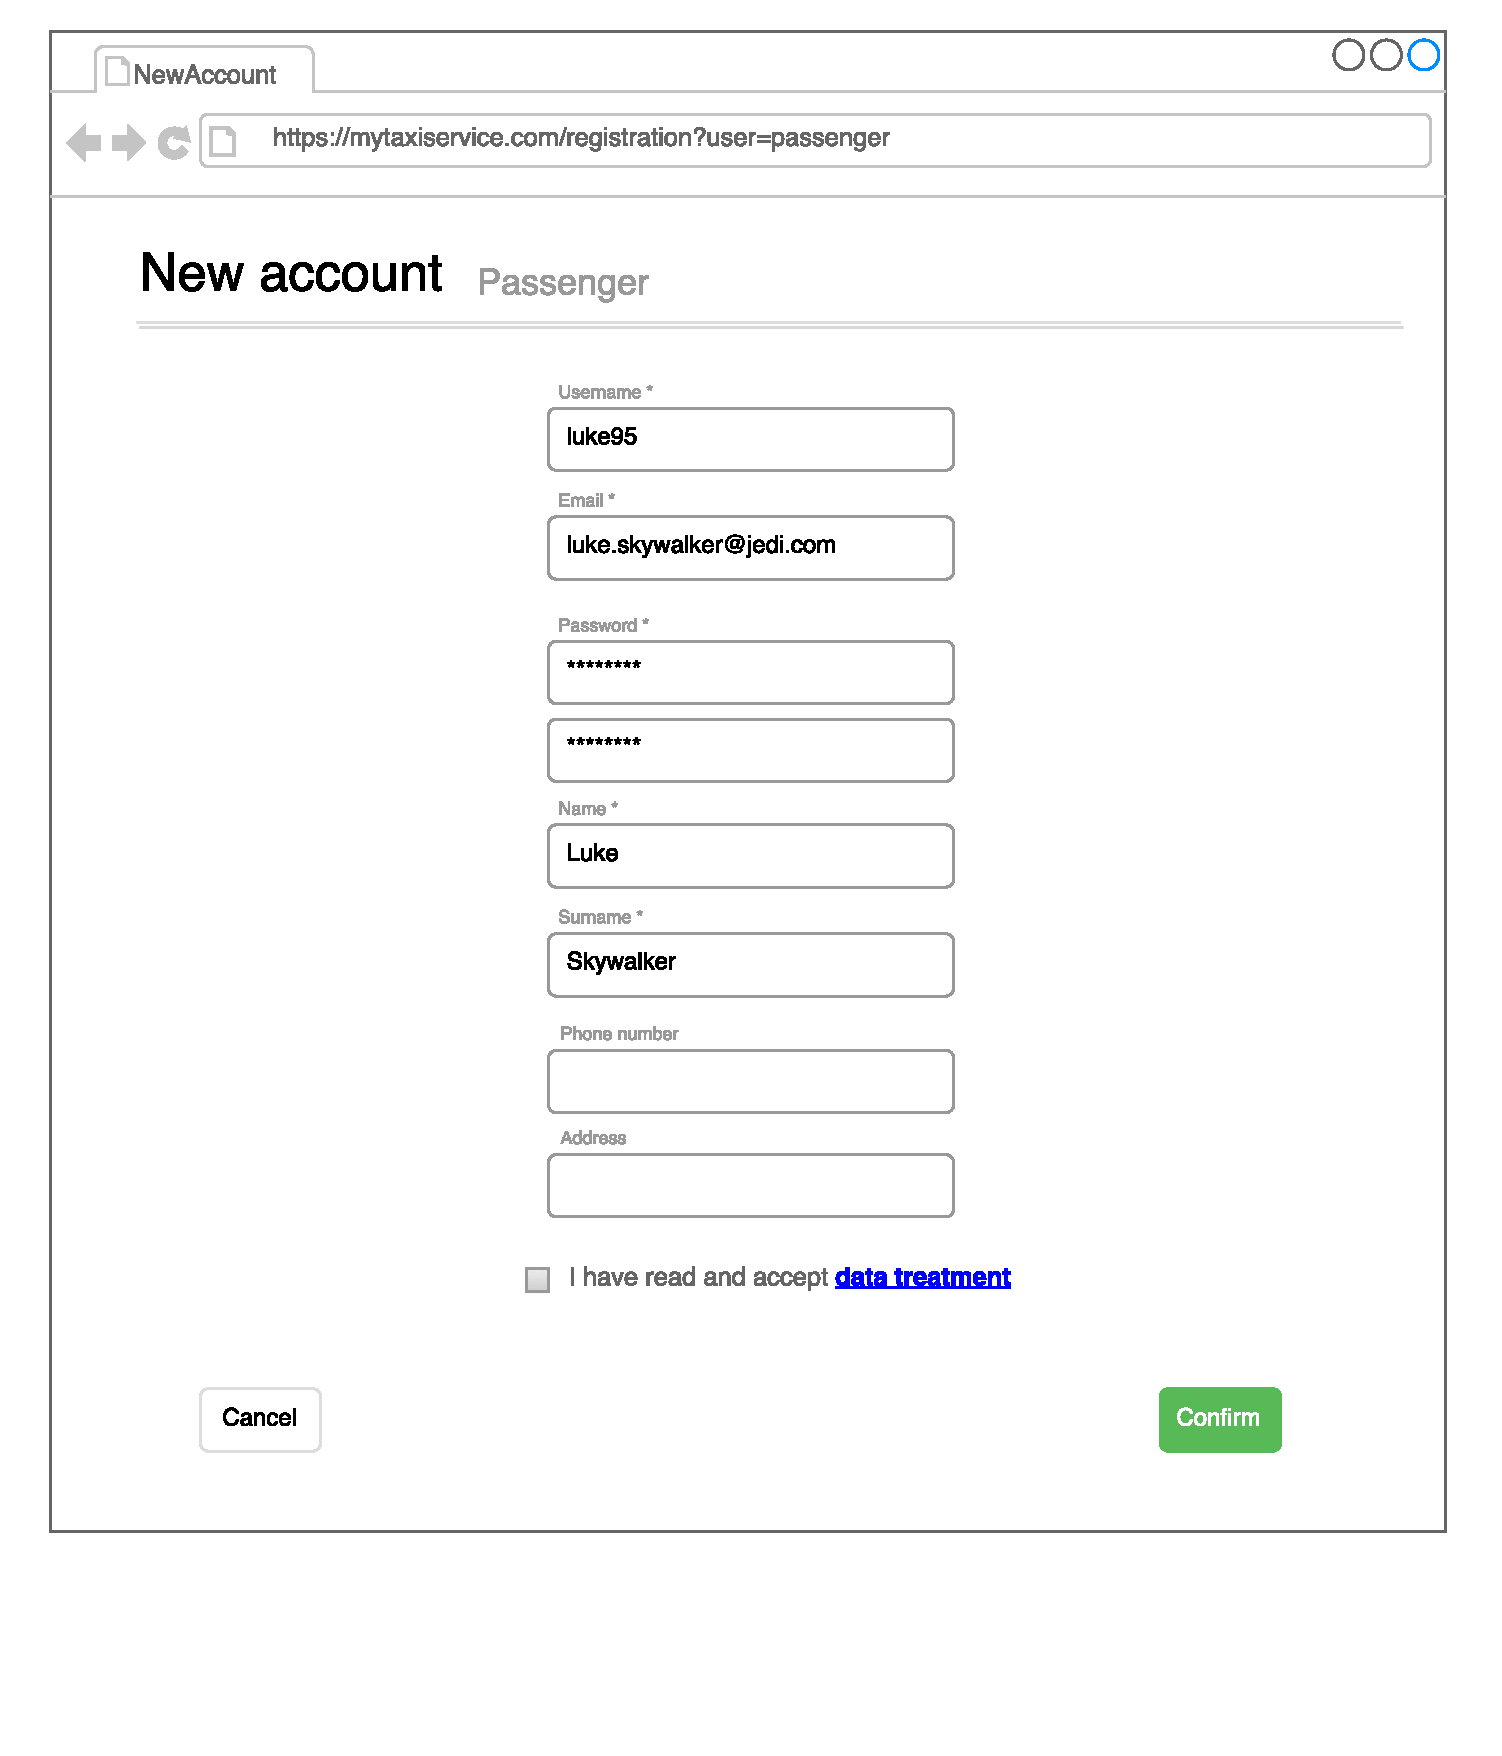
\includegraphics[width=\textwidth]{mockup/Registration.pdf}
\caption{Concept of the registration webpage.}
\label{fig:mockup-registration}
\end{figure}


\subsubsection{Use case}
The use case for user registration is shown in~\autoref{usecase-registration}.

\begin{table}
\begin{center}
\begin{tabular}{| l | p{0.6\textwidth} |}
\hline
Actor & Unregistered user, Registered passenger or taxi driver \\
\hline
Goal & Goal ~\ref{g-login}
\\
\hline
Input condition & The user chooses to create a new user account.  \\
\hline
Event Flow & \begin{enumerate}
	\item The user selects taxi driver or passenger registration.
	\item The registration form is loaded and the user compiles it.\label{load-registration}
	\item The user authorizes the personal data treatment.
	\item The user reads the e-mail received by myTaxiService and clicks on the link to confirm the registration.
	\end{enumerate}
\\
\hline
Output condition & The system tells the user that he/she has been successfully registered. \\
\hline

Exception &  \begin{itemize}
	\item Some exceptions are handled notifying the user of the problem and reloading the registration form (step~\ref{load-registration} of Event Flow).

	The requirements that generate these kind of exceptions are:
	\ref{f-sameInfo},    %The username/e-mail is already use by someone else.
	\ref{f-sameTaxi},   %The taxi license or number plate is already use by someone else.
	\ref{f-usrn},       %The username doesn't respect the restrictions.
	\ref{f-psw1},     %The password doesn't respect the restrictions.
	\ref{f-psw2}.    %The password entered the second time is different from the first one.
	\item Some exceptions are handled aborting the registration (all user's data is deleted).

	The requirements that generate these kind of exceptions are:
	\ref{f-dataTreat},   %The user doesn't authorises the data treatment.
	\ref{f-confirm}.   %The user doesn't confirms the registration clicking on the link received via e-mail.
	\end{itemize}
 \\
\hline
\end{tabular}
\end{center}
\caption{Use case for user registration.}
\label{usecase-registration}
\end{table}

\subsubsection{Statechart}
The statechart of the registration process is illustrated in figure \ref{fig:statechart-registration}.
\begin{figure}
\begin{center}
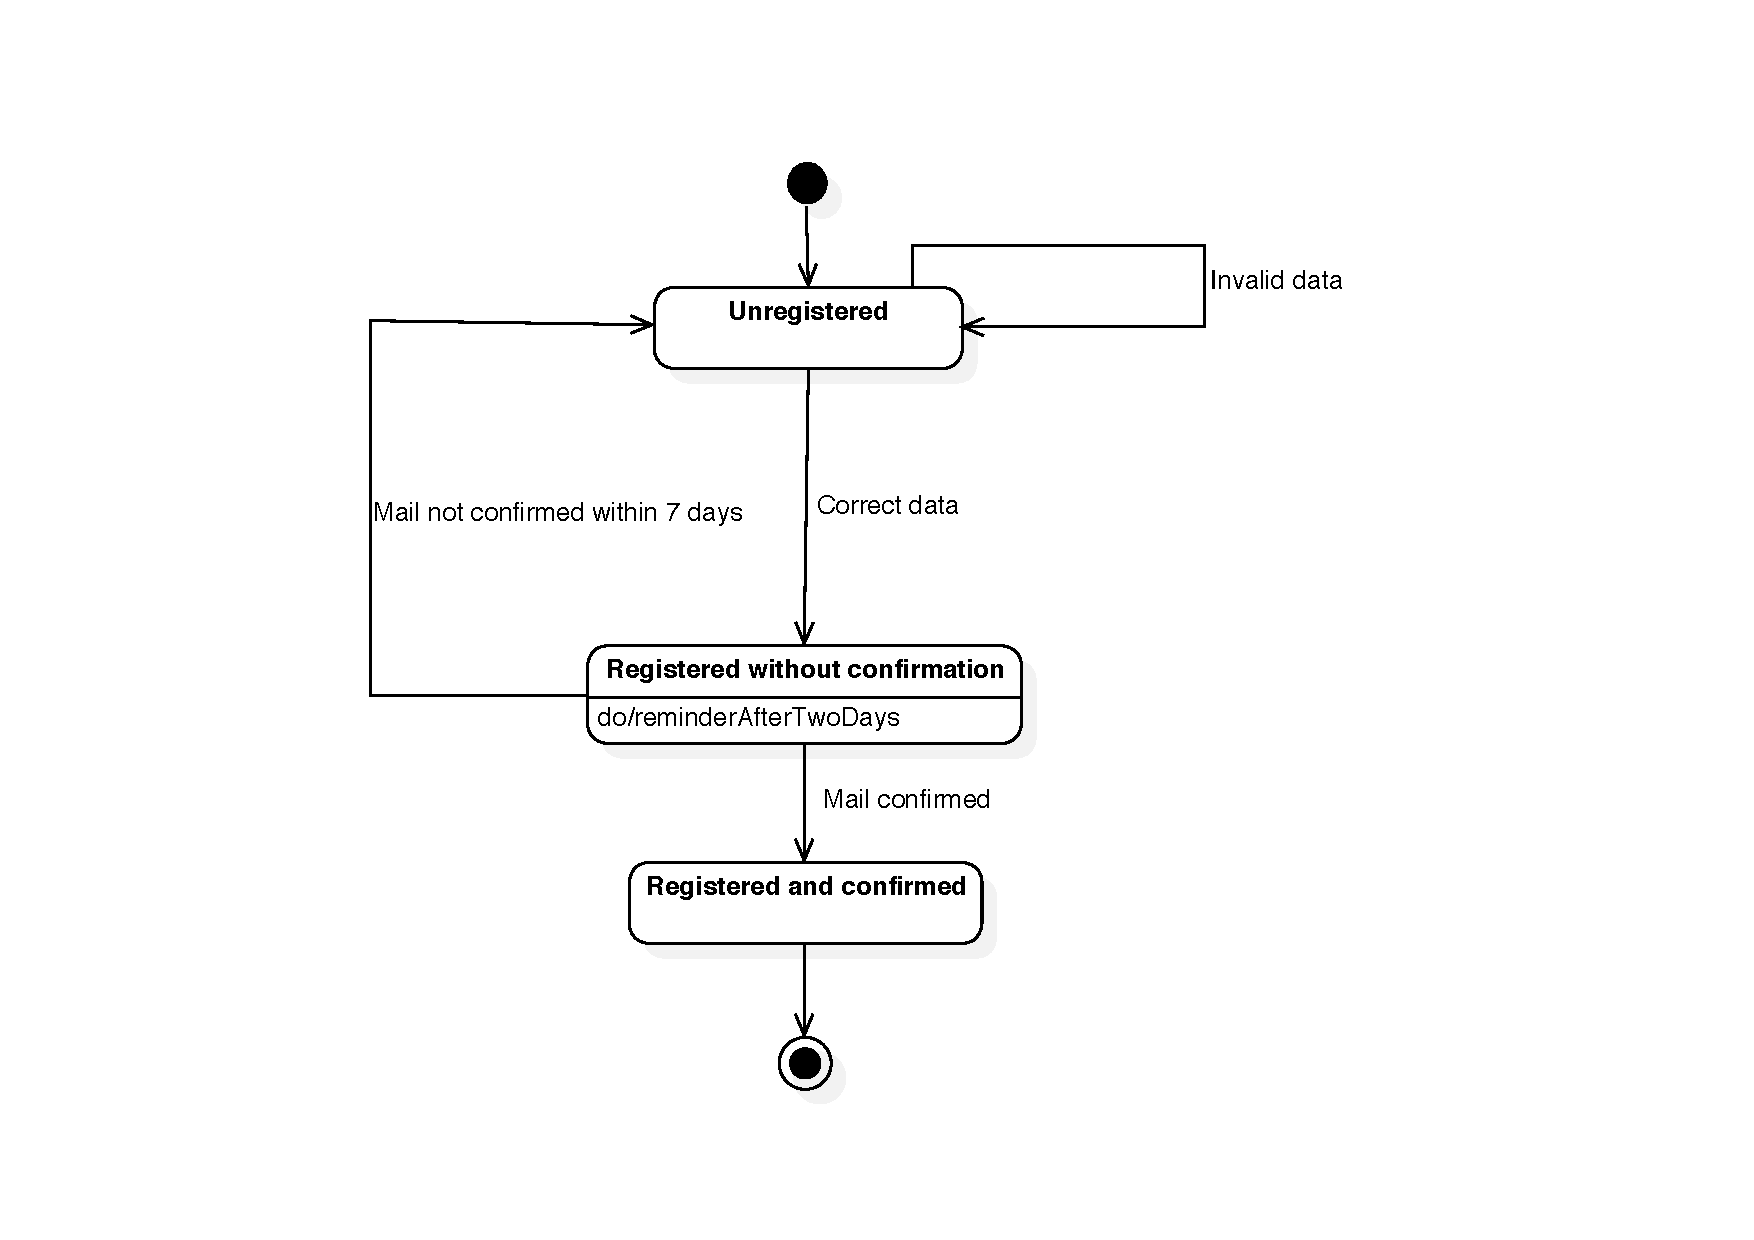
\includegraphics[width=0.7\textwidth]{diagrams/statechart_registration.pdf}
\caption{Statechart of the registration process.}
\label{fig:statechart-registration}
\end{center}
\end{figure}

\subsubsection{Associated functional requirements}

\begin{enumerate}
    \item On registration, the user can choose to register as a passenger or as a taxi driver.
    \item Passengers must provide the following information:
    \begin{itemize}
        \item e-mail address
        \item username
        \item password
        \item name
        \item surname
        \item address (optional filling)
        \item phone number (optional filling)
    \end{itemize}
    \item Taxi drivers must provide the following information:
    \begin{itemize}
        \item e-mail address
        \item username
        \item password
        \item name
        \item surname
        \item address
        \item phone number
        \item taxi license ID
        \item taxi number-plate
    \end{itemize}
    \item There mustn't be another user already subscribed with the same username or e-mail. \label{f-sameInfo}
    \item There mustn't be another taxi driver already subscribed with the same taxi license or taxi number plate. \label{f-sameTaxi}
    \item The username must match the regular expression\\``\texttt{[a-zA-Z][a-zA-Z0-9]\{2,20\}}''    \label{f-usrn}
    \item The system accepts a password that contains at least one number and one capital letter and that has a minimum length of eight characters.  \label{f-psw1}
    \item The system must ask for the password twice.
    \item The system accepts the password only if it is entered identically both times. \label{f-psw2}
    \item If the personal data treatment is not authorised, the subscription is canceled. \label{f-dataTreat}
    \item The system must allow the user to abort the registration process at any time.
    \item Email confirmation process:
    \begin{enumerate}
	    \item The subscription ends successfully when the user clicks on the link in the confirmation e-mail.
	    \item After two days without an answer, the systems sends another confirmation e-mail.
	    \item After seven days, the user's registration info are deleted and the user may re-try the registration process.  \label{f-confirm}
	\end{enumerate}
\end{enumerate}
